\chapter{Segunda forma fundamental, curvatura media y gaussiana}

\section{Segunda forma fundamental}
\large 

Sea una superficie parametrizada $S$,
\begin{align*}
    \mathbf{x}:U\subseteq \mathbb{R}^2&\longrightarrow V\cap S\\
    (u^1,u^2)&\longmapsto \mathbf{x}(u^1,u^2) \ ,
\end{align*}
y un punto genérico de la superficie $S$, $P$. Además, sea $T_p(S)$ el espacio o plano tangente a $S$ en el punto $P$. En este punto $P$, el conjunto de vectores $\left \{ \mathbf{x}_1=\pdv{\mathbf{x}}{u^1},\mathbf{x}_2=\pdv{\mathbf{x}}{u^2} ,\mathbf{n}=\frac{\mathbf{x}_1\wedge \mathbf{x}_2}{||\mathbf{x}_1\wedge \mathbf{x}_2||}\right \}$ es una base de $\mathbb{R}^3$.\\

\begin{wrapfigure}{l}{0.3\textwidth}
    \centering
    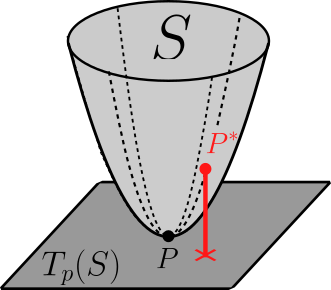
\includegraphics[scale=.5]{FOTOS/curvatura_dist.png}
\end{wrapfigure}

Consideramos un punto $P^*\in S$ infinitesimalmente próximo al punto $P$, de tal modo que las coordenadas de $P$ y $P^*$ son, respectivamente, $(u^1,u^2),(u^1+h^1,u^+h^2)$. Para medir la curvatura, estudiaremos cuánto se separa la superficie $S$ de $T_p(S)$.
$$
d(P^*,T_p(S))=(\mathbf{x}(u^p+h^p)-\mathbf{x}(u^p))\cdot \mathbf{n}
$$

Como $P$ y $P^*$ están infinitamente cerca, podemos expandir en serie de Taylor:
$$
\mathbf{x}(u^p+h^p)=\mathbf{x}(u^p)+\mathbf{x}_\alpha \cdot h^\alpha +\frac{1}{2}\mathbf{x}_{\alpha \beta }(u^p)\cdot h^\alpha h^\beta +\mathbf{R}_2
$$
Por lo que la distancia queda como:
\begin{equation*}
    \begin{split}
        d(P^*,T_p(S))&=\left ( \mathbf{x}_\alpha(u^p)\cdot h^\alpha +\frac{1}{2}\mathbf{x}_{\alpha \beta }(u^p)\cdot h^\alpha h^\beta +\ldots   \right )\cdot \mathbf{n}\\
        &=\frac{1}{2}\mathbf{x}_{\alpha \beta }\cdot \mathbf{n}h^\alpha h^\beta \qquad \text{porque }\mathbf{x}_\alpha \cdot \mathbf{n}=0
    \end{split}
\end{equation*}
Al producto escalar de la segunda derivada con el vector perpendicular a $T_p(S)$ lo llamaremos \emph{segunda forma fundamental}.
$$\boxed{b_{\alpha \beta }=\mathbf{x}_{\alpha \beta }\cdot \mathbf{n}}$$

Otra manera alternativa de expresar la segunda forma fundamental se obtiene derivando la expresión $\mathbf{x}_\alpha \cdot \mathbf{n}=0$:
$$
\mathbf{x}_{\alpha \beta }\cdot \mathbf{n}+\mathbf{x}_\alpha \mathbf{n}_\beta =0 \implies \boxed{b_{\alpha \beta }=-\mathbf{x}_\alpha \cdot \mathbf{n}_\beta }
$$

Para el determinante de esta matriz, utilizaremos la notación $b=\det{b_{\alpha \beta }}$. El nombre de segunda forma fundamental proviene de que la distancia $d(P^*,T_p(S))=1/2b_{\alpha \beta }h^\alpha h^\beta +\ldots $ es, a orden dominante, una forma cuadrática:
$$
Q(h^\alpha )=\frac{1}{2}b_{\alpha \beta }h^\alpha h^\beta 
$$

No obstante, al contrario que de la primera forma fundamental, esta \emph{no} tiene porqué ser definida positiva. 
\begin{mybox}
    \begin{center}
        \textbf{SEGUNDA FORMA FUNDAMENTAL}
    \end{center}
    $$
    b_{\alpha \beta }=\mathbf{x}_{\alpha \beta }\cdot \mathbf{n}=-\mathbf{x}_\alpha \cdot \mathbf{n}_\beta 
    $$
    \textbf{Propiedades:}
    \begin{enumerate}
        \item Si $b_{\alpha \beta }=0$ sobre una cierta carta local, la superficie en esa carta es un \textbf{plano}, y viceversa.
        \item $b_{\alpha \beta} $ son las componentes covariantes de un (pseudo-)tensor de segundo orden.
        \item La ley de transformación de $b$ es $\Bar{b}=D^2b$.
    \end{enumerate}
\end{mybox}
\begin{enumerate}
    \item[\fbox{1}] 
    \begin{proof}
            Suponemos que $b_{\alpha \beta }=0$, y sabemos que $||\mathbf{n}||=1 \leftrightarrow \mathbf{n}\cdot \mathbf{n}=1$. Derivando: $\mathbf{n}_\alpha \cdot \mathbf{n}+\mathbf{n} \cdot \mathbf{n}_\alpha\implies \mathbf{n}\cdot \mathbf{n}_\alpha =0 \iff \mathbf{n}_\alpha \in T_p(S)$. Esto significa que $\mathbf{n}_\alpha $ puede expresarse como combinación lineal de la base $\{ \mathbf{x}_1,\mathbf{x}_2 \} $. Por tanto:
            $$
            \left \{ \begin{array}{c}
                 b_{\alpha \beta }=0  \\
                 \mathbf{n}_\alpha \in T_p(S) 
            \end{array} \right . \implies \mathbf{x}_\alpha \cdot \mathbf{n}_\beta =0\iff \mathbf{n}\equiv \text{const.} 
            $$
            Entonces:
            $$
            (\mathbf{x}\cdot \mathbf{n})_\alpha =\cancelto{0}{\mathbf{n}\cdot \mathbf{x}_\alpha }+\cancelto{0}{\mathbf{n}_\alpha \cdot \mathbf{x}}
            $$
            Luego:
            $$
            \mathbf{x}\cdot \mathbf{n}\equiv \text{const.}\qquad \text{Ecuación de un plano.} 
            $$
    \end{proof}
    \item[\fbox{2}]
    \begin{proof}
        Si cambiamos de coordenadas $u^\alpha $ a $\Bar{u}^\beta $:
        \begin{equation*}
        \begin{split}
            \Bar{\mathbf{n}}=\frac{\Bar{\mathbf{x}}_1\wedge \Bar{\mathbf{x}}_2}{||\Bar{\mathbf{x}}_1\wedge \Bar{\mathbf{x}}_2||}\longrightarrow \Bar{b}_{\alpha \beta }=-\Bar{\mathbf{x}}_\alpha \cdot \Bar{\mathbf{n}}_\beta &=-\left ( \pdv{u^\mu }{\Bar{u}^\alpha } \mathbf{x}_\mu \right ) \cdot \left ( \pdv{u^\nu }{\Bar{u}^\beta } \mathbf{n}_\nu \right )\\
            &=- \pdv{u^\mu }{\Bar{u}^\alpha }\pdv{u^\nu }{\Bar{u}^\beta }\underbrace{\mathbf{x}_\mu\cdot \mathbf{n}_\nu}_{-b_{\mu \nu }}\\
            &=\pdv{u^\mu }{\Bar{u}^\alpha }\pdv{u^\nu }{\Bar{u}^\beta }b_{\mu \nu }
        \end{split}
        \end{equation*}
    \end{proof}
\end{enumerate}
\subsection{Clasificación de los puntos de una superficie}
Dada la superficie $S$, el plano tangente $T_p(S)$ y el punto $P^*$ de la superficie infinitesimalmente cerca de $P$, podemos clasificar las superficies en función de las diferentes separaciones del plano tangente.
\begin{itemize}
    \item \underline{PUNTO ELÍPTICO}: Si $b>0$, la superficie se comporta localmente como un paraboloide de revolución (o elíptico).
    $$
    Q(h^\alpha )=\frac{1}{2}b_{\alpha \beta }h^\alpha h^\beta 
    $$
    Además, si $b_{11}>0$, la superficie está orientada en el sentido de $\mathbf{n}$ (como el paraboloide elíptico, por ejemplo).\\
    Por el contrario, si $b_{11}<0$, la superficie está orientada en el sentido contrario a $\mathbf{n}$.

    \item \underline{PUNTO HIPERBÓLICO}: Si $b<0$, la superficie se comporta localmente como un paraboloide hiperbólico (punto de silla).
    \item \underline{PUNTO PARABÓLICO}: Si $b=0$ pero $b_{\alpha \beta }\neq 0$, la superficie se comporta localmente como un cilindro parabólico.
\end{itemize}

    \begin{wrapfigure}{r}{.3\textwidth}
    \centering
        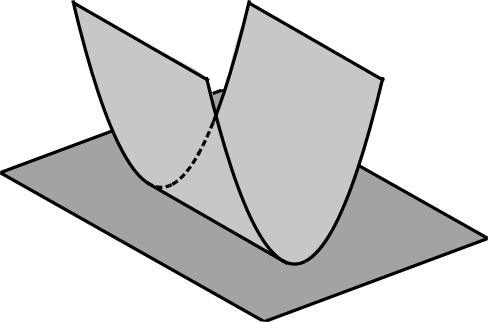
\includegraphics[scale=.3]{FOTOS/punto_parabolico.png}
        \caption*{Cilindro parabólico}
    \end{wrapfigure}
Si $b_{\alpha \beta}=0$ (es decir, la segunda forma fundamental se anula), entonces no podemos conocer la forma local de la superficie. En este caso, es necesario tomar el siguiente orden de aproximación en el desarrollo en serie de Taylor. A este tipo de puntos se les conoce como \underline{PUNTOS PLANARES}.\\

\WFclear
\begin{mybox}
\begin{wrapfigure}{r}{.36\textwidth}
        \centering
        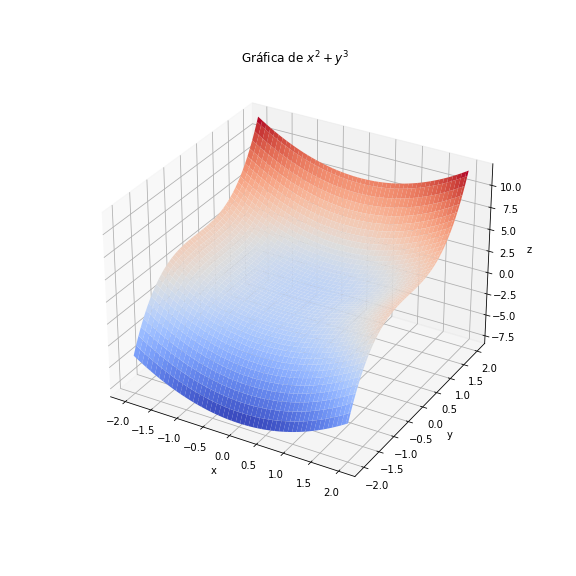
\includegraphics[scale=.3]{FOTOS/ejemplo3_A.png}
        \caption*{Gráfica de $f(x,y)=x^2+y^3$}
    \end{wrapfigure}
 \underline{Ejemplo A:} $\mathbf{x}(u^1,u^2)=(u^1,u^2,(u^1)^2+(u^2)^3)$
    
    $$\mathbf{x}_1=(1,0,2u^1),\ \mathbf{x}_2=(0,1,3(u^2)^2)$$
    $$
    \mathbf{n}=\frac{\mathbf{x}_1\wedge \mathbf{x}_2}{||\mathbf{x}_1\wedge \mathbf{x}_2||}=\frac{(-2u^1,-3(u^2)^2,1)}{\sqrt{1+(u^1)^2+9(u^2)^4}}
    $$
    $$
    b_{\alpha \beta }=\mathbf{x}_{\alpha \beta }\cdot \mathbf{n}
    $$
    $\implies 
    \left \{ \begin{array}{ccccc}
         \mathbf{x}_{11}&=&(0,0,2)&&  \\
         \mathbf{x}_{12}&=&(0,0,0)&=&\mathbf{x}_{21}\\
         \mathbf{x}_{22}&=&(0,0,6u^2)&&
    \end{array} \right .
    $\\
    $
    \implies \left \{ \begin{array}{ccccc}
         b_{11}&=&\frac{2}{\sqrt{1+(u^1)^2+9(u^2)^4}}&&  \\
         b_{12}&=&0&=&b_{21}\\
         b_{22}&=&\frac{6u^2}{\sqrt{1+(u^1)^2+9(u^2)^4}}&&\\
    \end{array} \right .\\
    $\WFclear$  \text{Es decir: \quad \parbox{8cm}{$b>0$ si $u^2>0$: puntos elípticos\\
                                                                 $b<0$ si $u^2<0$: puntos hiperbólicos\\
                                                                 $b=0$ si $u^2=0$: puntos parabólicos}}$
\end{mybox}

\section{Curvaturas principales, media y gaussiana}
\begin{wrapfigure}{l}{.35\textwidth}
    \centering
    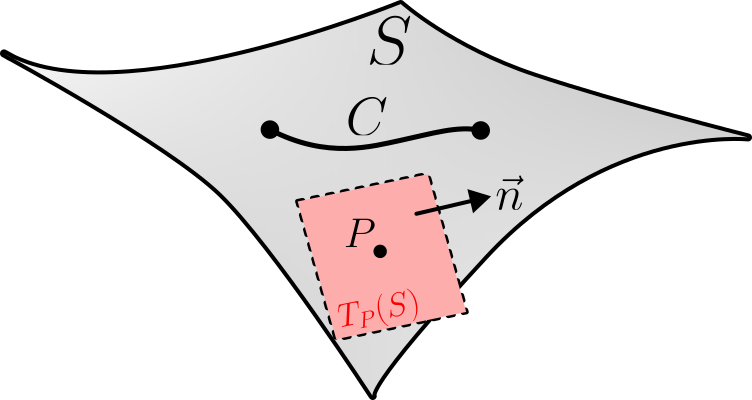
\includegraphics[scale=.26]{FOTOS/cpmg_1.png}
    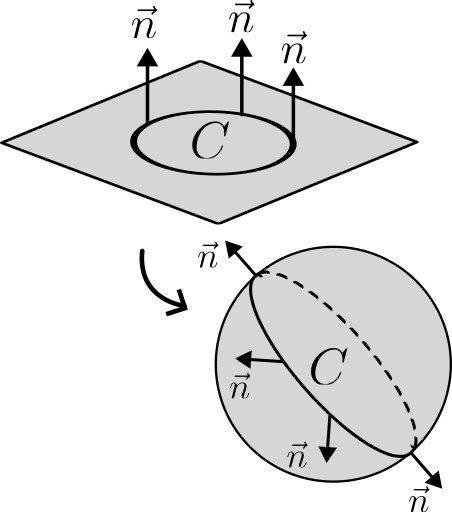
\includegraphics[scale=.35]{FOTOS/cpmg_2.png}
\end{wrapfigure}
La curvatura de una curva contenida dentro de una superficie dependerá de la propia curva y de la curvatura de la superficie. Como ejemplo, podemos pensar en una circunferencia contenida en un plano, o la misma circunferencia entendida como el ecuador de una esfera. \\

La contribución a la curvatura de la curva que proviene de la superficie se debe a cómo varía el vector normal sobre la superficie y, en concreto, del ángulo que forman entre $\mathbf{n}$ y $\mathbf{k}$, con $\mathbf{k}=k\cdot \mathbf{p}$, donde $\mathbf{p}$ es el vector normal principal de la curva. Para ver esto, descompondremos $\mathbf{k}$, el vector de curvatura, en una componente \emph{normal} (o paralela a $\mathbf{n}$); y en otra no paralela.\\
$$
\mathbf{k}=\mathbf{k}_n+\mathbf{k}_g \qquad \qquad \mathbf{k}_n\cdot \mathbf{n}=0 \ (\mathbf{k}_n\parallel \mathbf{n})
$$
$\mathbf{k}_g$ será entonces el vector de curvatura \emph{geodésica} (debida al tipo de curva). \\

Sea $S$ una superficie parametrizada, y $C$ una determinada curva en $S$, parametrizada en términos de la longitud de arco ($||\dot{\mathbf{x}}(S)||=1)$.
$$
\mathbf{k}_n=k_n\cdot \mathbf{n} \qquad \text{y} \qquad k_n=\mathbf{k}\cdot \mathbf{n}
$$
Como $\mathbf{k}$, para una curva en parámetro natural, es $\mathbf{k}=\dot{\mathbf{t}}=\ddot{\mathbf{x}}$; al aplicar la regla de la cadena queda:
\begin{gather*}
    \ddot{\mathbf{x}}=\pdv{\mathbf{x}}{u^\alpha }\dot{u}^\alpha =\mathbf{x}_{\alpha \beta }\dot{u}^\alpha \dot{u}^\beta +\mathbf{x}_\alpha \ddot{u}^\alpha \\
    \implies k_n=\ddot{\mathbf{x}}\cdot \mathbf{n}=(\mathbf{x}_{\alpha \beta }\dot{u}^\alpha \dot{u}^\beta +\mathbf{x}_\alpha \ddot{u}^\alpha)\cdot \mathbf{n}=b_{\alpha \beta }\dot{u}^\alpha \dot{u}^\beta 
\end{gather*}
En el caso de encontrarnos en una parametrización arbitraria:
$$
\dot{u}^\alpha =\dv{u^\alpha }{S}=\dv{u^\alpha }{t}\cdot \dv{t}{S}=(u^\alpha )'\cdot \frac{1}{||\mathbf{x}'(t)||}
$$
De esta forma, 
$$
k_n=\frac{1}{||\mathbf{x}'(t)||^2}b_{\alpha \beta }(u^\alpha )'(u^\beta)'=\boxed{\frac{b_{\alpha \beta }(u^\alpha )'(u^\beta )'}{g_{\mu \nu }(u^\mu )'(u^\nu )'}=k_n}
$$

La \emph{curvatura normal} es el cociente entre la segunda y la primera forma fundamental, evaluadas sobre la curva (conocidas $u^\alpha =u^\alpha (t)$). La curvatura normal es, en realidad, el ángulo entre $\mathbf{n}$ y el vector de curvatura $\mathbf{k}$ (o $\mathbf{p}$). \\
\newpage
\begin{wrapfigure}{r}{.35\textwidth}
    \centering
    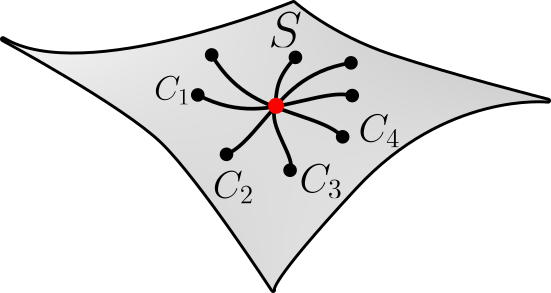
\includegraphics[scale=.37]{FOTOS/curva_normal.png}
\end{wrapfigure}
La curvatura de cada curva $C_i$ (las cuales pasan todas por el mismo punto), serán distintas, como aparece en la imagen. Para ello, definiremos las curvaturas normales principales de la superficie $S$ en el punto $P$.\\

\subsection{Curvaturas normales principales (de $S$ en $P$)}
Se definen como los valores mayor y menor de la curvatura normal para todas las curvas contenidas en esa superficie $S$ y que pasan por el punto $P$.\\

Por comodidad, introducimos la siguiente notación:
\paragraph{Notación:} $(u^\alpha )'=\dv{u^\alpha (t)}{t}=\ell ^\alpha \implies k_n=\frac{b_{\alpha \beta }\ell ^\alpha \ell ^\beta }{g_{\mu \nu }\ell ^\mu \ell ^\nu }=\frac{A}{B}$, con $A=b_{\alpha \beta }\ell ^\alpha \ell ^\beta $ y $B=g_{\mu \nu} \ell ^\mu \ell ^\nu $.\\

Para hallar los valores de $k_n$ máximos y mínimos, derivamos la curvatura normal e imponemos que sea nula.
$$
\pdv{k_n}{\ell ^\alpha }=0=\frac{B\pdv*{A}{\ell ^\alpha }-A\pdv*{B}{\ell ^\alpha }}{B^2}
$$
Si multiplicamos por $B$ y usamos que $k_n=A/B$, entonces la expresión anterior puede escribirse como:
$$
\pdv{A}{\ell^\alpha }-k_n\pdv{B}{\ell ^\alpha }=0
$$
y, junto con las expresiones explícitas de $A$ y $B$, llegamos a que:
$$
(b_{\alpha \beta }l^\beta +b_{\beta \alpha }\ell ^\beta )-k_n(g_{\alpha \beta }\ell ^\beta +g_{\beta \alpha }\ell ^\beta )=0
$$
Como $g_{\alpha \beta }$ y $b_{\alpha \beta}$ son simétricas en $\alpha $ y $\beta $, la expresión se simplifica:
\begin{gather*}
    (b_{\alpha \beta }-k_ng_{\alpha \beta})\ell ^\beta =0 \quad (\alpha ,\beta =1,2)\\
    \left .\begin{array}{cc}
         \alpha =1:&(b_{11}-k_ng_{11})\ell ^1+(b_{12}-k_ng_{12})\ell^2=0  \\
         \alpha =2:&(b_{21}-k_ng_{21})\ell ^1+(b_{22}-k_ng_{22})\ell^2=0
    \end{array} \right \} 
\end{gather*}
que es un sistema homogéneo con $(\ell^1,\ell^2)\neq (0,0)$. Por tanto, para las soluciones no triviales, el determinante de la matriz de coeficientes debe de ser nulo.
$$
\left | \begin{array}{cc}
     b_{11}-k_ng_{11}&b_{12}-k_ng_{12}  \\
     b_{21}-k_ng_{21}&b_{22}-k_ng_{22} 
\end{array} \right |=0
$$
Esta condición proporciona una ecuación con dos soluciones para $k_n$. Estas dos soluciones, que etiquetaremos $k_1$ y $k_2$ ($k_1\ge k_2$), se conocen como las \emph{curvaturas normales principales} de la superficie $S$ en el punto $P$.\\

Para calcular las curvaturas normales $k_1$ y $k_2$, introduciremos el \emph{operador de Weingarten}, que es la segunda forma fundamental con un índice covariante y otro contravariante.
$$
b^\mu {}_\nu \equiv \text{operador de Weingarten.}
$$
De la ecuación $(b_{\alpha \beta }-k_ng_{\alpha \beta})\ell ^\beta =0$, tenemos que 
\begin{gather*}
    g^{\alpha \mu}(b_{\alpha \beta }-k_ng_{\alpha \beta})\ell ^\beta =0\\
    \implies (b^\mu {}_\beta -k_n \delta ^\mu {}_\beta )\ell ^\beta =0\\
    \implies \left | \begin{array}{cc}
        b^1{}_1-k_n &b^1{}_2  \\
         b^2{}_1&b^2{}_2-k_n 
    \end{array} \right |=0
\end{gather*}
(que es una ecuación de autovalores para el operador de Weingarten). Desarrollando: 
$$
k_n^2-(b^1{}_1+b^2{}_2)k_n+(b^1{}_1b^2{}_2-b^2{}_1b^1{}_2)=0
$$
Si usamos que $b^1{}_1+b^2{}_2=b^\alpha {}_\alpha $ y que $\det(b^\mu {}_\nu )=\det(g^{\mu \alpha }b_{\alpha \nu})=\det(g^{\mu \nu })\det(b_{\alpha \nu})=b/g$, obtenemos la siguiente expresión:
$$
\boxed{k_n^2-b^\alpha {}_\alpha k_n+\frac{b}{g}=0}
$$

Las ecuaciones algebraicas de segundo grado pueden escribirse en términos de sus soluciones.
\begin{gather*}
    (k_n-k_1)(k_n-k_2)=0\\
    =k_n^2-(k_1+k_2)k_n+k_1k_2=0\\
    \implies k_1k_2=\frac{b}{g} \qquad k_1+k_2=b^\alpha {}_\alpha 
\end{gather*}

Y, finalmente, usando estas relaciones, podemos definir dos curvaturas para la superficie:
\begin{mybox}
    \begin{center}
        \textbf{CURVATURA MEDIA}
    \end{center}
    $$
    H\equiv \frac{1}{2}(k_1+k_2)=\frac{1}{2}b^\alpha {}_\alpha 
    $$
    Esta curvatura depende tanto de la primera forma fundamental como de la segunda forma fundamental.
    \begin{center}
        \textbf{CURVATURA GAUSSIANA}
    \end{center}
    $$
    K\equiv k_1\cdot k_2=\frac{b}{g}
    $$
    Al contrario de la curvatura media, esta curvatura \textbf{sólo depende de la primera forma fundamental}, al poder escribirse el determinante $b$ en términos de $g$.
\end{mybox}

A partir de esta definición, se dice que una superficie es \emph{minimal} si $H=0$ en todos sus puntos (el nombre se debe a que este tipo de superficies pueden probarse que tienen área mínima. Este es el caso del plano). Veamos cómo se transforman estas dos cantidades $H$ y $K$ bajo cambios de coordenadas. 

Como $b_{\alpha \beta }$ es un pseudo-tensor y $g_{\alpha \beta }$ es un tensor, $k_n$ sólo cambiará de signo si cambia el sentido de $\mathbf{n}$. Por tanto, el producto de $k_1k_2=K$ será \emph{invariante} bajo cambios de coordenadas. En consecuencia, la curvatura gaussiana $K$ es un \emph{escalar}. (también puede verse este hecho con las leyes de transformación tensoriales).
\section{Fórmulas de Weingarten y de Gauss. Símbolos de Christoffel}
Como hemos visto en el capítulo 1, el sistema de Frenet se adapta a la geometría de la curva que estudiamos (se desplaza con el parámetro $t$). La evolución de este sistema da lugar a la noción de curvaturas de una curva en $\mathbb{R}^n$. \\

En el caso de las superficies, escribiremos $\{ \mathbf{x}_{\alpha \beta },\mathbf{n}_\beta  \}$ en términos de $\{ \mathbf{x}_\alpha ,\mathbf{n} \}$, con $\alpha ,\beta =1,2$. Derivaremos los vectores $\{ \mathbf{x}_1,\mathbf{x}_2,\mathbf{n} \}$ con respecto a las coordenadas curvilíneas locales, 
$$
\mathbf{x}_{\alpha \beta }=\partial_\beta \mathbf{x}_\alpha =\Gamma_{\alpha \beta }{}^\gamma \mathbf{x}_\gamma +a_{\alpha \beta }\mathbf{n}
$$
$$
\mathbf{n}_\beta =\partial_\beta \mathbf{n}=c_\beta {}^\gamma \mathbf{x}_\gamma +d_\beta \mathbf{n}
$$
donde $\Gamma_{\alpha \beta}{}^\gamma ,a_{\alpha \beta} ,c_\beta ,d_\beta $ son los coeficientes. Analizamos primero la segunda ecuación: como $||\mathbf{n}||^2=\mathbf{n}\cdot \mathbf{n}=1,\ \mathbf{n}_\beta \cdot \mathbf{n}=0 \implies d_\beta =0$. 

Si usamos la base dual,
\begin{gather*}
    \mathbf{x}^\gamma \cdot \mathbf{n}_\beta =g^{\gamma \rho} \mathbf{x}_\rho \cdot \mathbf{n}_\beta=-g^{\gamma \rho} b_{\rho \beta }=-b^\gamma {}_\beta \\
    \implies \mathbf{x}^\gamma \cdot \mathbf{n}_\beta =c_\beta {}^\gamma =-b_\beta {}^\gamma 
\end{gather*}

De la primera ecuación, $\mathbf{n}\cdot \mathbf{x}_{\alpha \beta}=a_{\alpha \beta }$. Por definición, $b_{\alpha \beta }=\mathbf{n}\cdot \mathbf{x}_{\alpha \beta }$, de modo que $\mathbf{n}\cdot \mathbf{x}_{\alpha \beta }=a_{\alpha \beta }=b_{\alpha \beta }$. 

Si utilizamos la base dual, $\mathbf{x}^\gamma \cdot \mathbf{x}_{\alpha \beta }=\boxed{\Gamma _{\alpha \beta }{}^\gamma} $. Estas cantidades se conocen como los \emph{símbolos de Christoffel de segunda especie} (no son tensores). Los símbolos de Christoffel \emph{de primera especie} son:
$$
\Gamma _{\alpha \beta \gamma }=\mathbf{x}_\gamma \cdot \mathbf{x}_{\alpha \beta }=g_{\mu \gamma }\Gamma ^\mu{}_{\alpha \beta }
$$

La notación usada en la literatura matemática es $\Gamma _{\alpha \beta }{}^\gamma $. En física--y, en concreto, en Relatividad General-- usamos la notación $\Gamma ^\gamma {}_{\alpha \beta }$. \\

Con esta definición, las ecuaciones anteriores pueden escribirse como:
\begin{align}
    \mathbf{x}_{\alpha \beta }&=\Gamma _{\alpha \beta }{}^\gamma \mathbf{x}_\gamma +b_{\alpha \beta }\mathbf{n} &&\text{: Ecuación de Gauss} \tag*{[G]} \label{gauss}\\
    \mathbf{n}_\beta &=-b_\beta {}^\gamma \cdot \mathbf{x}_\gamma &&\text{: Ecuación de Weingarten} \tag*{[W]} \label{weingarten}
\end{align}
$$
b_{\alpha \beta }=\mathbf{n}\cdot \mathbf{x}_{\alpha \beta } \qquad \qquad \Gamma _{\alpha \beta }{}^\gamma =\mathbf{x}^\gamma \cdot \mathbf{x}_{\alpha \beta }
$$
\section{Propiedades de los símbolos de Christoffel}
\subsection{Simetrías}
Del \emph{teorema de Schwarz} \footnote{Básicamente, si $f(x,y)$ es continua en su dominio abierto $D$ y es de clase $C^2$, entonces $f_{xy}=f_{yx}$.}, $\mathbf{x}_{\alpha \beta }=\mathbf{x}_{\beta \alpha }$, con $\alpha ,\beta =1,2$, luego los símbolos de Christoffel, $\Gamma _{\alpha \beta }{}^\gamma =\mathbf{x}^\gamma \cdot \mathbf{x}_{\alpha \beta }$ son simétricos bajo el intercambio de $\alpha $ y $\beta $.
$$
\Gamma _{\alpha \beta }{}^\gamma =\Gamma _{\beta \alpha  }{}^\gamma 
$$
Esto significa que, de los $2\times 2\times 2=8$ símbolos posibles en un superficie, sólo 6 de ellos son independientes (en dimensión $n$, serían $n^2(n+1)/2$).\\

Gracias a esta simetría, es posible obtener los símbolos de Christoffel en términos de derivadas de la primera forma fundamental. Esta expresión será la definición más común para estos símbolos. \\

Habíamos definido la primera forma fundamental como:
$$
g_{\alpha \lambda }=\mathbf{x}_\alpha \cdot \mathbf{x}_\lambda ,\ \text{con }\alpha ,\lambda=1,2.
$$
Si derivamos con respecto a $u^\beta $:
\begin{equation} \label{[*]}\tag*{[*]}
    \begin{split}
        \pdv{g_{\alpha \lambda  }}{u^\beta }&=\mathbf{x}_{\alpha \beta }\cdot \mathbf{x}_\lambda +\mathbf{x}_\alpha \cdot \mathbf{x}_{\lambda \beta }\\
        &=\Gamma_{\alpha \beta \lambda }+\Gamma _{\lambda \beta \alpha }
    \end{split}
\end{equation}
Si ahora rotamos los índices cíclicamente: $\alpha \rightarrow \beta \rightarrow \lambda \rightarrow \alpha $
\begin{equation} \label{[**]}
    \pdv{g_{\beta \alpha }}{u^\lambda }=\Gamma _{\beta \lambda }+\Gamma _{\alpha \lambda \beta } \tag*{[**]}
\end{equation}
\begin{equation}\label{[***]}
    \pdv{g_{\lambda \beta }}{u^\alpha }=\Gamma _{\lambda \alpha \beta }+\Gamma _{\beta \alpha \lambda }\tag*{[***]}
\end{equation}
Si ahora calculamos \ref{[*]}+\ref{[***]}-\ref{[**]}:
$$
\pdv{g_{\alpha \lambda  }}{u^\beta }+\pdv{g_{\lambda \beta }}{u^\alpha }-\pdv{g_{\beta \alpha }}{u^\lambda }=2\Gamma _{\alpha \beta \lambda }
$$
Por lo que, finalmente, podemos escribir:
$$
\boxed{\Gamma _{\alpha \beta \lambda }=\frac{1}{2}\left ( \pdv{g_{\alpha \lambda  }}{u^\beta }+\pdv{g_{\lambda \beta }}{u^\alpha }-\pdv{g_{\beta \alpha }}{u^\lambda } \right )}
$$
que es la definición para los símbolos de Christoffel de primera especie. \\

Para los símbolos de Christoffel de segunda especie, usamos la primera forma fundamental en notación contravariante.
\begin{mybox}
    \begin{center}
        \textbf{DEFINICIÓN DE SÍMBOLOS DE CHRISTOFFEL}
    \end{center}
    De primera especie:
    $$
    \Gamma _{\alpha \beta \lambda }=\frac{1}{2}\left ( \pdv{g_{\alpha \lambda  }}{u^\beta }+\pdv{g_{\lambda \beta }}{u^\alpha }-\pdv{g_{\beta \alpha }}{u^\lambda } \right )
    $$
    De segunda especie:
    $$
    \Gamma _{\alpha \beta }{}^\mu =g^{\mu \lambda }\Gamma _{\alpha \beta \lambda }=\frac{1}{2}g^{\mu \lambda }\left ( \pdv{g_{\alpha \lambda  }}{u^\beta }+\pdv{g_{\lambda \beta }}{u^\alpha }-\pdv{g_{\beta \alpha }}{u^\lambda } \right )
    $$
    \noindent\rule{\textwidth}{0.5pt}
    \underline{Ejemplo B:}
    \begin{enumerate}
        \item[(i)] Símbolos de Christoffel para coordenadas ortogonales sobre una superficie $S$.
        $$
        g_{\alpha \beta }=g_{\alpha \beta }(u^1,u^2)=\left ( \begin{array}{cc}
             g_{11}&  \\
             & g_{22}
        \end{array} \right )\rightarrow g^{\alpha \beta }=\left ( \begin{array}{cc}
             1/g_{11}&  \\
             & 1/g_{22}
        \end{array} \right )
        $$
        Los símbolos de Christoffel son $\Gamma _{11}{}^1=g^{1\lambda }\Gamma _{11\lambda }$.
        \begin{equation*}
            \begin{split}
                \Gamma _{11}{}^1&=g^{11}\Gamma_{111}+\cancel{g^{12}\Gamma _{112}}=\frac{1}{2g_{11}}\left ( \pdv{g_{11}}{u^1}+\cancel{\pdv{g_{11}}{u^1}}-\cancel{\pdv{g_{11}}{u^1}} \right )\\
                &=\frac{1}{2g_{11}}\pdv{g_{11}}{u^1}(u^1,u^2)
            \end{split}
        \end{equation*}
        \begin{gather*}
            \Gamma _{22}{}^1=-\frac{1}{2g_{11}}\pdv{g_{22}}{u^1} ,\quad \Gamma_{11}{}^2=-\frac{1}{2g_{11}}\pdv{g_{11}}{u^2} ,\quad \Gamma_{22}{}^2=\frac{1}{2g_{22}}\pdv{g_{22}}{u^2} \\
            \Gamma_{12}{}^1=\Gamma_{21}{}^1=\frac{1}{2g_{11}}\pdv{g_{11}}{u^2},\quad \Gamma_{12}{}^2=\Gamma_{21}{}^2=\frac{1}{2g_{22}}\pdv{g_{22}}{u^1}
        \end{gather*}

        \item[(ii)] Símbolos de Christoffel para el plano en coordenadas polares:\\
        $
        \mathbf{x}(u^1,u^2)=(u^1\cos u^2,u^1 \sin u^2,0) \quad (r,\theta)
        $
        $$
        g_{\alpha \beta }=\left ( \begin{array}{cc}
            1 &  \\
             & (u^1)^2
        \end{array} \right )=\left ( \begin{array}{cc}
             1&  \\
             &r^2 
        \end{array} \right )
        $$
        $$
        \Gamma_{22}{}^1=\Gamma_{rr}{}^\theta =-r ,\quad \Gamma_{12}{}^2=\Gamma_{21}{}^2=\Gamma_{r\theta}{}^\theta =\Gamma_{\theta r}{}^\theta =1/r
        $$
    \end{enumerate}
\end{mybox}
Una relación útil de los símbolos de Christoffel es la de la contracción de símbolos:
$$
\Gamma_{\alpha \beta }{}^\alpha =\frac{1}{2}g^{\alpha \lambda}\left ( \pdv{g_{\alpha \lambda}}{u^\beta }+ \cancel{\pdv{g_{\beta  \lambda}}{u^\alpha }}-\cancel{\pdv{g_{\alpha \beta}}{u^\lambda  }}\right )=\frac{1}{2}g^{\alpha \lambda}\pdv{g_{\alpha \lambda }}{u^\beta }
$$
Otra relación útil es la siguiente:
$$
\pdv{g}{u^\beta }=\pdv{}{u^\beta }\left (g_{11}g_{22}-(g_{12})^2\right )=\partial_\beta g_{11} g_{22}+g_{11}\partial_\beta g_{22}-2g_{12}\partial_\beta g_{12}
$$
Además: $g_{\alpha \beta }=\left ( \begin{array}{cc}
     g_{11}&g_{12}  \\
     g_{21}& g_{22}
\end{array} \right )\Rightarrow  g^{11}=g_{22}/g,\ g^{22}=g_{11}/g$, $g^{12}=g^{21}=-g_{12}/g$, luego:
$$
\partial_\beta g=gg^{11}\partial_\beta g_{11}+gg^{22}\partial_\beta g_{22}+2gg^{12}\partial_\beta g_{12}=gg^{\alpha \lambda} \pdv{g_{\alpha \lambda }}{u^\beta }
$$
Combinando los dos resultados:
$$
\boxed{\Gamma_{\alpha \beta }{}^\alpha =\frac{1}{2g}\pdv{g}{u^\beta }=\pdv{}{u^\beta }[\log \sqrt{g}]}
$$
\subsection{Ley de transformación de los símbolos de Christoffel}
$(U,\mathbf{x}(u^\alpha )\longrightarrow (\Bar{U},\Bar{\mathbf{x}}(\Bar{u}^\alpha )$: Al cambiar de parametrización:
$$
\Bar{\mathbf{x}}_\alpha =\pdv{u^\gamma }{\Bar{u}^\alpha }\mathbf{x}_\gamma  \quad , \quad \Bar{\mathbf{x}}^\lambda =\pdv{\bar{u}^\lambda }{u^\sigma }\mathbf{x}^\sigma 
$$
La segunda derivada cumple:
$$
\Bar{\mathbf{x}}_{\alpha \beta }=\pdv{}{\Bar{u}^\beta }\Bar{\mathbf{x}}_\alpha =\pdv{u^\gamma }{\Bar{u}^\alpha }\pdv{u^\mu }{\Bar{u}^\beta }\mathbf{x}_{\gamma \mu }+\pdv{u^\gamma }{\Bar{u}^\alpha }{\Bar{u}^\beta }\cdot \mathbf{x}_\gamma 
$$
Es decir, los símbolos de Christoffel (de segunda especie) en las nuevas coordenadas (carta $(\Bar{U},\Bar{\mathbf{x}}(\Bar{u}^\alpha ))$) son:
\begin{equation*}
    \begin{split}
        \Bar{\Gamma }_{\alpha \beta }{}^\lambda =\Bar{\mathbf{x}}_{\alpha \beta }\cdot \Bar{\mathbf{x}}^\lambda &=\color{red}\pdv{u^\gamma }{\Bar{u}^\alpha }\pdv{u^\mu }{\Bar{u}^\beta }\pdv{\Bar{u}^\lambda }{u^\sigma }\overbrace{\mathbf{x}_{\gamma \mu }\cdot \mathbf{x}^\sigma }^{\Gamma_{\gamma \mu }{}^\sigma }\color{blue} +\pdv{u^\gamma }{\Bar{u}^\alpha }{\Bar{u}^\beta }\pdv{\Bar{u}^\lambda }{u^\sigma }\underbrace{\mathbf{x}_\gamma \cdot \mathbf{x}^\sigma }_{\delta_\gamma {}^\sigma }\\
        &=\color{red}{\pdv{u^\gamma }{\Bar{u}^\alpha }\pdv{u^\mu }{\Bar{u}^\beta }\pdv{\Bar{u}^\lambda }{u^\sigma }\Gamma_{\gamma \mu }{}^\sigma }\color{blue} +\pdv{u^\gamma }{\Bar{u}^\alpha }{\Bar{u}^\beta }\pdv{\Bar{u}^\lambda }{u^\sigma }
    \end{split}
\end{equation*}
El término en rojo corresponde a la ley de transformación tensorial habitual. El término azul 'estropea' este carácter tensorial de los símbolos de Christoffel (salvo reparametrizaciones lineales).
\section{Tensor de curvatura de Riemann}
Ahora deduciremos las \emph{ecuaciones de Mainardi-Codazzi}. Como hemos visto, a través de la superficie parametrizada podemos deducir información acerca de la curvatura de ésta:
$$
\mathbf{x}(u^1,u^2)\longrightarrow \mathbf{x}_\alpha =\partial _\alpha \mathbf{x}\longrightarrow g_{\alpha \beta }=\mathbf{x}_\alpha \cdot \mathbf{x}_\beta \longrightarrow \mathbf{n}\longrightarrow b_{\alpha \beta }\longrightarrow g,b,H,K\longrightarrow \Gamma _{\alpha \beta }{}^\gamma  
$$

Las ecuaciones de Mainardi-Codazzi establecen, fundamentalmente, que $\mathbf{x}_{\alpha \beta \gamma}=\mathbf{x}_{\alpha \gamma \beta }$, que es la condición de integrabilidad. Esto hace que la superficie no tenga ninguna obstrucción o patología, y existe una independencia sobre el camino que tomamos integrando entre dos puntos infinitesimalmente próximos. \\

Si derivamos la fórmula de Gauss, \ref{gauss}:
\begin{gather*}
    \mathbf{x}_{\alpha \beta }=\Gamma _{\alpha \beta }{}^\gamma \mathbf{x}_\gamma +b_{\alpha \beta }\mathbf{n}\implies \mathbf{x}_{\alpha \beta \gamma }=\pdv{}{u^\gamma }\mathbf{x}_{\alpha \beta }\\
    \pdv{}{u^\gamma }\mathbf{x}_{\alpha \beta }=\partial_\gamma \Gamma_{\alpha \beta}{}^\sigma \cdot \mathbf{x}_\sigma +\Gamma_{\alpha \beta}{}^\sigma \cdot \mathbf{x}_{\sigma \gamma }+\partial_\gamma b_{\alpha \beta }\cdot \mathbf{n}+b_{\alpha \beta }\cdot \mathbf{n}_\gamma
\end{gather*}
Y si ahora usamos la fórmula de Weingarten, \ref{weingarten}: $\mathbf{n}_\gamma =-b_\gamma {}^\sigma  \cdot \mathbf{x}_\sigma $, y la de Gauss:
\begin{equation*}
    \begin{split}
        \mathbf{x}_{\alpha \beta \gamma }&=\partial_\gamma \Gamma _{\alpha \beta }{}^\sigma \mathbf{x}_\sigma +\Gamma _{\alpha \beta }{}^\sigma \left ( \Gamma _{\sigma \gamma }{}^\rho \mathbf{x}_\rho +b_{\sigma \gamma }\cdot \mathbf{n} \right )+\partial_\gamma b_{\alpha \beta }\cdot \mathbf{n}-b_{\alpha \beta }b_\gamma {}^\sigma \mathbf{x}_\sigma \\
        \mathbf{x}_{\alpha \beta \gamma  }&=\left ( \partial_\gamma \Gamma _{\alpha \beta }{}^\sigma+ \Gamma _{\sigma \gamma }{}^\rho \Gamma _{\rho \gamma }{}^\sigma -b_{\alpha \beta} b_\gamma {}^\sigma \right )\cdot \mathbf{x}_\sigma +\left ( \Gamma _{\alpha \beta } {}^\sigma b_{\sigma \gamma }+\partial_\gamma b_{\alpha \beta } \right )  \cdot \mathbf{n}
    \end{split}
\end{equation*}
Como $\{ \mathbf{x}_\alpha ,\mathbf{n} \}$ son vectores linealmente independientes, al imponer la condición de $\mathbf{x}_{\alpha \beta \gamma }=\mathbf{x}_{\alpha \gamma \beta }$, los términos que vayan con cada vector deben ser idénticamente iguales, obteniéndose dos conjuntos de ecuaciones, que son las ecuaciones de Mainardi-Codazzi.
\begin{gather*}
    \pdv{\Gamma_{\alpha \beta }{}^\sigma }{u^\gamma }-\pdv{\Gamma _{\alpha \gamma }{}^\sigma }{u^\beta }+\Gamma _{\alpha \beta} {}^\rho\Gamma _{\rho \gamma }{}^\sigma -\Gamma _{\alpha \gamma }{}^\rho \Gamma _{\rho \beta }{}^\sigma =b_{\alpha \beta }b_\gamma {}^\sigma -b_{\alpha \gamma }b_\beta {}^\sigma \\
    \Gamma _{\alpha \beta }{}^\sigma b_{\sigma \gamma }-\Gamma _{\alpha \gamma }{}^\sigma b_{\sigma \beta }+\pdv{b_{\alpha \beta }}{u^\gamma }-\pdv{b_{\alpha \gamma }}{u^\beta }=0
\end{gather*}
\subsection{Tensor de curvatura de Riemann}
Analizando la primera ecuación de M-C, el lado derecho es un producto de segundas formas fundamentales. La segunda forma fundamental, $b_{\alpha \beta }=\mathbf{x}_{\alpha \beta }\cdot \mathbf{n}$, es un pseudo-tensor. El producto da lugar, por tanto, a algo que se comporta de forma \emph{tensorial}. En este caso, esto hace que sea un tensor de cuarto orden, tres veces covariante y una vez contravariante. \\

Por definición, el lado izquierdo de la primera ecuación se conoce como el \emph{tensor de curvatura de Riemann}.
$$
\boxed{R^\sigma {}_{\alpha \gamma \beta }\equiv \pdv{\Gamma_{\alpha \beta }{}^\sigma }{u^\gamma }-\pdv{\Gamma _{\alpha \gamma }{}^\sigma }{u^\beta }+\Gamma _{\alpha \beta} {}^\rho\Gamma _{\rho \gamma }{}^\sigma -\Gamma _{\alpha \gamma }{}^\rho \Gamma _{\rho \beta }{}^\sigma}
$$
Para presentar las simetrías del tensor de Riemann, trabajaremos con su versión cuatro veces covariante.
$$
R_{\mu \alpha \gamma \beta }=g_{\mu \sigma }R^\sigma {}_{\alpha \gamma \beta }=b_{\alpha \beta }b_{\gamma \mu} -b_{\alpha \gamma }b_{\beta \mu}
$$
Este tensor cumple las siguientes propiedades:
\begin{itemize}
    \item $R_{\mu \alpha \ \gamma \beta }= R_{ \gamma \beta \ \mu \alpha}$ (simetría por pares de índices)
    \item $R_{\mu \alpha  \gamma \beta }=-R_{\alpha  \mu  \gamma \beta }$ (antisimetría en los dos primeros índices)
    \item $R_{\mu \alpha  \gamma \beta }=-R_{\mu \alpha   \beta \gamma}$ (antisimetría en los dos últimos índices)
    \item $R_{\mu \alpha  \gamma \beta }+R_{\mu  \beta  \alpha  \gamma}+R_{\mu   \gamma \beta \alpha}=0$ (propiedad cíclica)
\end{itemize}

La construcción $R^\sigma {}_{\alpha \gamma \beta }$ es general, válida en dimensión $n$. Sus simetrías nos permiten reducir el número de componentes independientes a $n^2(n^2-1)/12$. En nuestro caso, $n=2$, una componente independiente. Las propiedades vistas anteriormente permiten reducir las componentes independientes de $n^4(n^2-1)/12$ a $n^2(n^2-1)/12$.
\section{Teorema egregio de Gauss}
Dada la superficie $\mathbf{x}(u^1.u^2)$, podemos calcular $g_{\alpha \beta }\rightarrow \Gamma_{\mu \nu }{}^\rho \rightarrow R^\mu {}_{\nu \sigma \rho}$. En el caso de $n=2$, tiene $n^2(n^2-1)/12=1$ componente individual. De hecho, sus únicas componentes distintas de 0 son $R_{1212}=R_{2121}=-R_{1221}=-R_{2112}$. Además, $R_{\mu \alpha \gamma \beta }=b_{\alpha \beta} b_{\gamma \mu}-b_{\alpha \gamma }b_{\beta \mu }$, y sustituyendo nos queda:
$$
R_{1212}=b_{22}b_{11}-b_{21}b_{21}=b_{11}b_{22}-(b_{12})^2=b
$$

Para $n=2$, $R_{1212}=b$. Y, si recordamos que la curvatura gaussiana se calcula como $K=k_1k_2=b/g$:
$$
\boxed{K=\frac{R_{1212}}{g}}
$$

Este resultado se conoce como el \emph{teorema egregio de Gauss}. Este teorema, fundamentalmente, establece que la curvatura gaussiana \emph{solo depende de la primera forma fundamental}, como hemos visto anteriormente.\\

El teorema egregio nos proporciona una vía alternativa y rápida para calcular el tensor de Riemann de una superficie sin necesidad de obtener los símbolos de Christoffel.
\begin{align*}
\mathbf{x}(u^1,u^2)\longrightarrow b_{\alpha \beta }\xlongrightarrow{\text{det}}&\text{\parbox{9cm}{\begin{center}
    Tensor de Riemann (4 veces covariante) ($n=2, R_{1212}$)
\end{center}}}\\
\xlongrightarrow{g^{\sigma \mu }} &\ \ \text{Tensor de Riemann } R^\sigma {}_{\alpha \gamma \beta }
\end{align*}
\paragraph{Comentarios:} 
\begin{itemize}
   \item El teorema egregio de Gauss (\emph{Theorema Egregium} en latín) establece que la curvatura de una superficie únicamente depende de la primera forma fundamental, como hemos visto anteriormente. Otra formulación distinta del teorema egregio es que la curvatura gaussiana es \emph{invariante bajo isometrías}, ya que bajo isometrías se preservan los elementos de matriz de $g_{\alpha \beta }$. Una consecuencia de esto es que no se puede realizar una transformación de una esfera, con curvatura gaussiana constante de $1/r^2$, a un plano sin que conlleve una distorsión de ángulos y distancias; es decir, sin que cambie su curvatura.

    \item Otros tensores importantes derivados del tensor de Riemann son el \emph{tensor de Ricci}, que se define como $R_{\mu \nu}=R^\alpha {}_{\mu \alpha \nu }$; y el \emph{tensor de Einstein} $G_{\mu \nu }=R_{\mu \nu }-1/2 g_{\mu \nu } R$, con $R=R_\mu {}^\mu $ el \emph{escalar de curvatura de Riemann}.   
\end{itemize}
